\chapter{The Fractal Objects Architectural Pattern}\label{ch01:00}

\myepigraph{Things which any idiot could write usually have the quality of having been written by an idiot.}{Bram Cohen}

  In his speech at the NDC~2012 conference, Robert Martin stated that there was no significant improvements to the processes of software construction comparing to the results in object-oriented analysis of the 1990th. 
  Even more, in his experience, today a large percentage of companies often regard a set of tools for software development to be equivalent to an architecture of a software system.
  This misconception is reinforced by the existence of multiple frameworks and libraries that on the one hand significantly facilitate the software development, but on the other hand completely shadow the actual architecture and purpose of software systems\footnote{Terms \emph{software systems} and \emph{software application} are used interchangeably.}.

  An influential work by Ivar~Jacobson~\cite{jacobson1992} provided an approach for designing a software architecture and implementing the core business functionality independently from any specific technology such as a web framework or some communication protocol.
  One of the intents of this approach was to enable easy migration of the core functionality (the business value) to any new or different software technology.
  That in turn should ensure longevity of that core functionality without changing it while the supporting technologies (e.g. frameworks, protocols) could change at a rapid pace.

  However, Jacobson's approach has two distinctive limitations that together make it not suitable for all situations:  
  \begin{enumerate}
   \item The architectural part of the core functionality that provides a way to tap into the supporting technology (i.e. boundaries) significantly complicates the development process.
   \item The use case approach limits capabilities of the application by enforcing a rigid behaviour.
  \end{enumerate}
  
  The first limitation forces developers to keep changing implementation for boundaries whenever either the supporting technology or the core business functionality changes.
  It does seem to be a necessary evil to separate software architecture from supporting technologies.
  However, could there be a better approach?  
  In order to make this limitation more obvious let's consider a not too far stretched comparison where there would be a need to change some part of a Java application related to automatic memory management whenever either some business logic needs to be changed or a new garbage collector is introduced into JVM.
  Instead, a computing platform such as JVM, provides an automatic memory management in a non-intrusive way for applications it executes.
  This kind of abstraction is required at an application level that would follow the information hiding principle to segregate the surrounding technology from its core functionality.
  
  The second limitation is related to the first whereby the concept of boundaries obstructs the business model from end-users.
  Interestingly, this is done intentionally and all interactivity between the system and end-users happens within the scope of predefined use cases.
  This corresponds to the \emph{conversational metaphor} as defined in~\cite{HHN1986}, which is natural for process-oriented software systems\footnote{A popularity of process orientation seems to be related to a wide spread adoption of the imperative programming paradigm that heavily influences the overall design of software systems, including UI.}.
  
  Obstructing the underlying business model complicates reasoning about a software system by end-users and impedes communication between them and developers.  
  The \emph{world model metaphor}~\cite{HHN1986} emphasises the importance of transparency of the business model in the UI, so that end-users could directly interact with that model without any intermediaries.
  The application of the world model metaphor to the system design has been researched by Richard Pawson~\cite{pawson2001, pawson2004}.
  This research resulted in creation of an architectural pattern and a framework called Naked Objects.
  The Naked Objects pattern reinforces the MVC pattern by promoting domain-oriented style for capturing the business model (M) and supporting an automatic generation of UI (VC) from that model.
  By employing domain-orientation for modelling, Naked Objects falls into the category of domain-driven design~\cite{haywood2009} that provides an alternative to Jacobson's approach for system design~\cite{evans2003, vernon2013}.
  
  However, neither Naked Objects nor other known to us domain-driven frameworks offer an approach that would address the problem of software system design and construction from the perspective of conceptual modelling of information systems.
  From a conceptual modelling perspective each system should provide three functions~\cite{oli2007}: 
  \begin{description}
    \item[\textbf{Memory.}] Maintains a representation of the state of a domain.
    \item[\textbf{Informative.}] Provides information about the state of a domain.
    \item[\textbf{Active.}] Perform actions that change the state of a domain. 
  \end{description} 
  In order to design and construct a holistic software system, its architecture should incorporate these three essential functions.

  This section discusses an approach implemented in the Trident Genesis platform called Fractal Objects. 
  It follows the \emph{participatory modelling} trend in conceptual modelling of information systems, which is typical for domain-oriented approaches, but has an inherent support for all three functions of an information system.  
  Structurally Fractal Objects represents an object-oriented data model that consists of the \emph{definition} and \emph{manipulation} languages.
  
  A well suited area of application for Fractal Objects (similar as for other domain-driven design approaches) is transactional business applications such as Enterprise Resource Planning (ERP) and Enterprise Asset Maintenance (EAM) systems.
  Therefore, many details of the following discussion are best understood in (but not limited to) the context of transactional business applications.
  
\section{Fractal Objects Model}

  In theory of data modelling, a conceptual data model is defined as a pair of languages~-- a data definition language and a data manipulation language~\cite{kal1983}.
  This definition is used in relational data modelling and both languages are incorporated into the SQL standard.
  Having a data model described in terms of SQL allows one to easily move this model and associated data instances between different RDBMS system with very little if any changes.
  At the same time concrete RDBMS implementations are very specific, have their own algorithms and optimisations techniques to effectively manage the data described by such generic models.
  This demonstrates the power of the conceptual data model that is desirable for any information system.
  
  We claim that a similar conceptual model can be effectively applied for modelling information systems using general-purpose object-oriented languages.
  Such model should have a language to describe business domain and a language for manipulation of objects that are described with the first language.
  Then there should be a computing platform that could run any concrete domain model similarly to an RDBMS system that can run any concrete data model described with SQL.
  This role of such computing platform is implemented in a form of the Trident Genesis platform.
  
  The main purpose of such platform is to abstract out the technologies required to run the resulting software system.
  We had very specific requirements to the computing platform that would ensure the robustness of the approach.
  The most important of them are formulated as the following traits:
  \begin{itemize}
    \item The dependency between the platform and the model should only exist in the sense that the platform ``understands'' both the definition and manipulation languages used for modelling a business domain.
    \item The platform should segregate the details of persistence and communication mechanism.
    \item The platform should provide an automatic generation of UI from the model that would follow the direct manipulation principle and support customisation.
  \end{itemize}

  Fig.~\ref{img:ch02:01:domain-integration} schematically depicts the integration between an application specific domain model and the platform running it.
  Through the use of specialised internal DSLs, type system and metadata for defining a domain model, the platform is provided with a capability to interpret the model at runtime for fulfilling all three essential functions of an information system. 
  The following discussion delves more into the details of this integration.

  \begin{figure}[!htp]
     \centering
    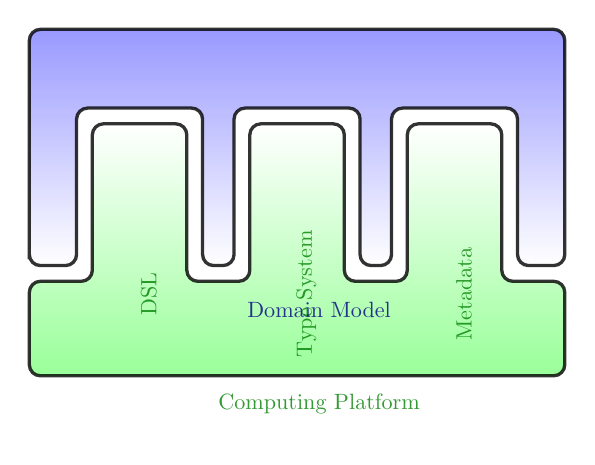
\begin{tikzpicture}[scale=0.8,  every node/.style={transform shape}, node distance=1cm, auto, opacity=0.8]
      \tikzset{
	  application/.style={rectangle,rounded corners,draw=black, top color=blue!50!white, bottom color=white,very thick, inner sep=1em, minimum size=3em, text centered, text=blue!50!black},
	  platform/.style={rectangle,rounded corners,draw=black, top color=white, bottom color=green!50!white,very thick, inner sep=1em, minimum size=3em, text centered, text=green!50!black},
	  mylabel/.style={text width=7em, text centered} 
      }  
      
      \def\platformpath{-- +(8.5cm,0cm) -- +(8.5cm,1.5cm) -- +(7.5cm,1.5cm) -- +(7.5cm,4.0cm) -- +(6.0cm,4.0cm) -- +(6.0cm,1.5cm) -- +(5.0cm,1.5cm) -- +(5.0cm,4.0cm) -- +(3.5cm,4.0cm) -- +(3.5cm,1.5cm) -- +(2.5cm,1.5cm) -- +(2.5cm,4.0cm) -- +(1.0cm,4.0cm) -- +(1.0cm,1.5cm) -- +(0.0cm,1.5cm) -- cycle}
      
      \draw (-1,-1.5) [platform] \platformpath
	    node [below, text width=3.5cm, text centered, yshift=1.0cm, xshift=1.15cm, rotate=90] {DSL}
	    node [below, text width=3.5cm, text centered, yshift=1.0cm, xshift=3.65cm, rotate=90] {Type System}
	    node [below, text width=3.5cm, text centered, yshift=1.0cm, xshift=6.15cm, rotate=90] {Metadata}
	    node [below, text centered,xshift=4.4cm, yshift=-0.2cm] {Computing Platform};

      \def\apppath{-- +(0cm,0cm) -- +(0.75cm,0cm) -- +(0.75cm,2.5cm) -- +(2.75cm,2.5cm) -- +(2.75cm,0cm) -- +(3.25cm,0cm) -- +(3.25cm,2.5cm) -- +(5.25cm,2.5cm) -- +(5.25cm,0cm)-- +(5.75cm,0cm)-- +(5.75cm,2.5cm) -- +(7.75cm,2.5cm) -- +(7.75cm,0cm) -- +(8.5cm,0cm) -- +(8.5cm,3.75cm) -- +(0cm,3.75cm) -- cycle}

      \draw (-1,0.25) [application] \apppath node [above, text centered,xshift=4.4cm, yshift=-1.2cm] {Domain Model};
    \end{tikzpicture} 
    \caption{Integration of Domain Model with the Platform}\label{img:ch02:01:domain-integration} 
  \end{figure}
    
  \subsection{The Definition Language}

  It was our intention to restrict the definition language to the expressive capabilities of a general-purpose object-oriented language (Java in this case).
  Thus, instead of developing an external DSL for domain model definition, a pure object-oriented approach of using a set of specifically designed classes together with meta-data capabilities of Java was developed that provides all the essential facilities for defining domain models.
  Rich type systems of modern object-oriented languages together with meta-data support provide very comprehensive means to capture domain information in a statically typed manner that is superior to relational data structures.  
  The business domain entities are modelled by reusing the type system provided in the platform, which supports well-defined patterns for modelling real-life interoperability between domain entities.  

  \begin{wrapfigure}{r}{0.4\textwidth}
    \vspace{-20pt}
    \centering   
    \begin{tikzpicture}[>=latex']
      \tikzset{
	  outercore/.style={circle, fill=blue!50!white, inner sep=0em, minimum size=2.3cm},
	  core/.style={circle, shade, ball color=green!50!white, inner sep=0em, minimum size=1.3cm},
      }      
      \begin{scope}[opacity=0.8]
	\node (o) at (0, 0) [outercore, opacity=0.3] {};	
	\node (c) at (0, 0) [core] {};
% 	\node at (0, -1.8cm) [text=blue!50!black] {Domain Entity Model};
      \end{scope}

      \node (ot) at (1.3, 1.5) [text=green!50!black,scale=0.8] {Entity Type};	
      \fill [green!50!black,->,out=220,in=80] (ot.south) edge (c.north);
      \node (ct) at (-1.3, 2) [text=blue!50!black,scale=0.8] {Metadata};	
      \fill [blue!50!black,->,out=-100,in=150] (ct.south) edge (o.west);      
    \end{tikzpicture} 
    \caption{Entity Object Model}\label{img:ch02:02:entity-object-model}
  \end{wrapfigure}  
  The meta-data provides a declarative way to associate various business rules (e.g. validation rules) with domain entities, define application security, control transaction demarcation, visual representation of domain entities and more.
  It also assists in the fine-tuning of the business domain models with the support of configuration-based behaviour that is achieved by means of dependency injection.  
  Based on runtime type information and meta-data, the platform can automatically construct a large portion of the application internals that provides support for the complete application life-cycle.
  For instance, the provided meta-data and types are sufficient for automatic construction of the application user interface that can leverage the validation rules and dependencies between domain entities.  
  Fig.~\ref{img:ch02:02:entity-object-model} schematically depicts a domain entity model.

  \subsubsection{Entity and Companion Objects}
  
  A Fractal Object is a pair $\langle E, C\rangle$, where $E$ is an \emph{entity object} and $C$ is a \emph{companion object}.
  \emph{Entity object} models a concrete entity from a business domain (WorkOrder, Vehicle etc.).
  Its purpose is to capture the structure of a domain entity it models~-- properties and associations with other domain entities.  
  Entity objects should have no behaviour, which is unlike other approaches such as Naked Objects where behaviour is an essential part of domain objects.
  Properties in an entity object that has a type of some other or the same entity object represents an relationship between these entity objects.
  Relationships between entity objects can either be one-to-one, many-to-one or one-to-many where the property type is a collection of entity objects.
  It is important to note that from the perspective of class hierarchy, the hierarchy of entity objects is flat~-- the complexity of the domain is captured via the composition mechanism rather than inheritance.  
  Changing relationship between domain entities at runtime can be achieved by simply changing values of their respective properties~-- something that cannot be done where association is captured through mechanism of inheritance.
  
  \emph{Companion object} defines four groups of operations that can be performed with respect to a corresponding entity object.  
  Each companion object is tightly coupled with a corresponding entity object and cannot be used for any other.
  The four groups of operations are: \emph{create}, \emph{save}, \emph{delete} and \emph{request}.
  The power of having a very limited number of operations has been demonstrated by the REST style~\cite{Fie2000} of architecture for web applications.
  We argue that similar benefits can be achieved at the level of domain modelling.
  There is a lot of semantic similarities between REST style of web resources (macro level) and objects modelling the domain (micro level).
  For example, the use of URI paths to navigate between web resources is analogous to paths in object graphs for association traversal.
  To us this resonates with an original view of object-oriented systems by Alan Key, who emphasised similarity between objects and networked computers.
  And although web is just a delivery mechanism, and a software system may or may not run on the web, its intrinsic nature of interconnected resources with uniform interaction mechanism seems to be very appropriate for an object-oriented modelling.
  It was one of our design goals to capture this approach of modelling complex structures and behaviour as the Fractal Objects design pattern.

  Having four groups of operations does not restrict the number of methods for a companion object.
  It only requires that all methods should be implemented as combinations of those four basic groups of operations to provide higher level of abstraction.
  Similarly to entity objects, companion objects can be composed in order to achieve a more complex behaviour.
  Companion objects provide a clean separation of concern by fully encapsulating the behaviour, making sure that entity objects represent a pure structure that is modelling the relationships between entities in a business domain.

  Thus, Fractal Objects are the primitives that by means of composition and the application of four basic groups of operations can model complex structures and behaviour.
  
  \subsubsection{Kinds of Fractal Objects}

  In order to implement the three essential functions of an information system, Fractal Objects provide three metaphors (kinds of fractal objects):
  \begin{description}
    \item[\textbf{Persistent Entities.}] A fractal object that models a domain entity that should maintain a persistent state.
    \item[\textbf{Synthesised Entities.}] A fractal object that is based on (synthesised) several persistent entities or subset of their properties.
    \item[\textbf{Functional Entities.}] A fractal object used to model a use case that involves one or more persistent entities.
  \end{description}

  \begin{wrapfigure}{r}{0.43\textwidth}
    \centering    
    \begin{tikzpicture}[>=latex']
      \tikzset{
	  outercore/.style={circle, fill=blue!50!white, inner sep=0em, minimum size=0.6cm},
	  core/.style={circle, shade, ball color=green!50!white, inner sep=0em, minimum size=0.3cm},
	  score/.style={circle, fill=green!50!black, inner sep=0em, minimum size=0.3cm},
	  outer/.style={circle, fill=blue!50!white, inner sep=0em, minimum size=2.3cm},
      }
      \begin{scope}[opacity=0.8]
	\node (o) at (0, -0.25) [outer, opacity=0.3] {};      
	\fill[circle, color=green!50!white] (0, -0.25) circle (0.7cm) node [below,text=blue!50!black,yshift=1.1cm] {};
      \end{scope}
      
      \begin{scope}[scale=0.3,opacity=0.8]
	\node (t) at (0,0) [outercore, opacity=0.5] {};	
	\node at (0,0) [core, opacity=0.5] {};

	\node (r) at (1,-1.2) [outercore, opacity=0.5] {};	
	\node at (1,-1.2) [core, opacity=0.5] {};

	\node (l) at (-1,-1.2) [outercore, opacity=0.5] {};	
	\node at (-1,-1.2) [score] {};
      \end{scope}
      
      \node (pe) at (1.3, 1.5) [text=green!50!black,scale=0.8] {Persistent Entities};      
      \fill [green!50!black,->,out=-100, in=80] (pe.south) edge (t.north);
      \fill [green!50!black,->,out=-100,in=80] (pe.south) edge (r.north);
      
      \node (se) at (-1.3, 2) [text=blue!50!black,scale=0.8] {Synthesised Entity};
      \fill [blue!50!black,->,out=-60,in=160] (se.south) edge (l.west);
      \node (se) at (-3.3, 1) [text=orange!50!black,scale=0.8] {Functional Entity};
      \fill [orange!50!black,->,out=-80,in=160] (se.south) edge (o.west);      
    \end{tikzpicture} 
    
     \caption{Composition of fractal objects}\label{img:ch02:03:fractal-objects-composition}
  \end{wrapfigure}
  
  Most business applications require the majority of domain entities to be stored for future reference or analyses.
  Such domain entities are modelled with so-called \emph{persistent} entity types.
  However, not all domain entities need to be persisted.
  One of the unique domain modelling concepts of Fractal Objects is that of \emph{synthesised} and \emph{functional} entities, which allow modelling of short-lived domain entities in exactly the same way as persistent entities.
  These kinds of entities can mix in any other kind, which is especially powerful when there is a need to combine loosely coupled domain entities as a single business concept or a usecase.
  This provides a uniform way for implementing business processes that may involve all three kinds of entities.
  Please note that synthesised and functional entities may have a persistent nature.
  For example, a functional entity modelling some specific use case may persist information what domain entities have been modified during its execution, who and when performed it etc.

  In principle these kinds of fractal objects are almost identical except some meta-data information, and can be composed without any restriction to form complex structures and behaviour.
  Fig.~\ref{img:ch02:03:fractal-objects-composition} schematically depicts a functional entity that is composed of one synthesised entity and two persistent entities.
  When a save operation is applied to such fractal object, it actions, which may lead to modification of a persistent state for persistent entities it incorporates.

  \subsection{The Manipulation Language}

  The four basic groups of operations, which are introduced at the companion object level together with capabilities of the Java programming language to modify state of objects at runtime, provide a way to manipulate the sate of the modelled domain.
  The platform provides support for a persistence mechanism that implements basic operations \emph{save} and \emph{delete}.
  However, there is a need for a comprehensive manipulation language similar in power to the data retrieval capabilities of SQL in order to support implementation for the \emph{request} group of basic operations.
  The main requirement for such language was its object-orientation that would naturally fit the modelling capabilities of entity objects, and would provide object-retrieval capabilities based on constraints applied to any part of the object graph.

  As the result an internal DSL called \emph{Entity Query Language}~(EQL) has been developed.
  The choice of an internal DSL was made in light of the fact that it is easy to remedy its computational limitations by tapping into the power of general-purpose language it is built with\footnote{
  Also, it followed our firm belief that implementation of an information system should be done using one programming language as opposed to many modern technologies that require utilisation of multiple diverse languages.
  This is especially true for current web technologies.}.

  Despite a recent surge of NoSQL databases, the vast majority of transactional business applications depend on RDBMS systems that provide the most adequate solution for managing data in such domains.
  In fact, many researches show that NoSQL capabilities are mainly applicable in the domains where there is a lot of poorly structured data such as documents, while Enterprise domains are best represented with a proper model that captures structural aspects and relational dependencies.
  Thus, Trident Genesis utilises RDBMS as its storage mechanism and provides translation of EQL queries into SQL.

  In order to better describe the role of \emph{Entity Query Language}, it is presented in contrast to object-relational mapping frameworks~(ORM).
  The main emphasis in modern ORM frameworks is heavily shifted towards approaches for the best mapping of object-oriented concepts such as classes, inheritance, encapsulation to the relational concept (sets and relations)~\cite{Barnes:2007:ORM, HBBPB:2008}.
  This area is well developed and there are industry wide initiatives for producing an API standard similar to SQL.
  One of such standards is Java Persistence API (JPA)~\cite{DeMichiel:2012:JPA}, which has a vibrant community and dynamic adaptation by many vendors.
  
  However, there is still a lot of debate about advantages and disadvantages of ORM solutions~\cite{Neward:2006:VCS, Fowler:2012:OH}.
  One of the weakest aspect of ORM remains its limitation of data querying capabilities that are significantly behind its relational counterpart~-- Structured Query Language.
  We suggest that the reason for this lies in the way transactional business applications are structured:
  \begin{itemize}
   \item ORM frameworks are used mainly as an easy way to start developing front-end applications, which are frequently build using OOP languages, to quickly tap into some relational database.
   Usually, such applications have rather rudimentary support for analytical features that could require a comprehensive querying mechanism. 
   At the same time front-end applications are used by the majority of corporate end-users who enter data into the system.
   \item In most cases powerful analytical capabilities are provided by external business intelligence tools.
   The problem with these tools is that they completely ignore the application layer (i.e. the domain model expressed in object-oriented terms) and instead work directly with the underlying database.
  \end{itemize}
  Existing technologies such as Hibernate, EclipseLink, Microsoft Entity Framework have a limited data querying support.
  And while ORM frameworks try to hide relational nature of databases, their querying mechanisms still very closely resemble relational operators from SQL.
  
  The holistic approach to the information system modelling is essential for making sustainable applications that could fulfil the needs of different groups of users.
  One of the evident proofs of this is the emerging concept of \emph{Embedded Business Intelligence} that brings analytical capabilities back to the core system~\cite{XLSHW2007}.
  This concept offers instant decision making and immersive user experience, and its implementation requires a holistic information system design with proper domain modelling and information retrieval function~\cite{oli2007}.
  A fully capable data querying mechanism is an inherent building block of such systems.
  In our view this should be achieved by close integration between the domain model and the querying mechanism that would allow tapping into the knowledge it captures.

\paragraph{Object graph traversal.}

  Object composition serves as a way for modelling relationships between domain entities in OOP~\cite{Martin2002}, and is re-enforced in Fractal Objects.
  Thus, if it is necessary to access an object property in the context of some other object the notion of \emph{dot-notated property path} is used, where the dot symbol (aka \emph{navigation operator}~\cite{DeMichiel:2012:JPA}) separates properties from each other.
  Dot-notated paths represent paths in object graphs stored in computer memory and provide an essential mechanism for accessing data represented as objects.
  Therefore, traversal of dot-notated paths from the relational perspective is one of the key aspect for data querying.
  Current ORM frameworks translate dot-notated paths into a series of INNER JOIN operators, which are applicable only to non-collectional composition\footnote{Composition representing only many-to-one and one-to-one associations, many-to-zero and one-to-zero are also not supported.}.
  The developed as part of Trident Genesis model for relation traversal supports automatic selection of the most appropriate strategy~-- INNER JOIN, OUTER JOIN, EXISTS and their combination.
  This is achieved by close integration with the underlying domain model and its meta-data in conjunction with high level query language (Entity Query Language~\cite{Hodych:2012}) that is implemented as an internal DSL based on progressive interfaces~\cite{Fowler:2010:DSL}.

  \lstset{morekeywords={val,select,where,prop,eq,and,begin,end,starts_with,any_of_values,values,or,yield_and_group,as,yield,begin_expr,sum_of,div,end_expr,model,in,sumOf,with,gt,modelAs, modelAsAggregate, groupByAndYield, within, prevMonth},
  numbers=left, numberstyle=\tiny, stepnumber=1, numbersep=5pt,
  basicstyle=\scriptsize\color{basiccolor}, keywordstyle=\bfseries\color{codefgcolor}, stringstyle=\color{stringcolor}}

  \begin{code}{Entity query example (aggregation)}{\label{ch01:00:lst:eql-aggregation}}{codebgcolor}
    \begin{lstlisting}
select(Vehicle.class).
where().
  prop("vehModel.make").eq().val("MERCEDES").
  and().
  sumOf().prop("fuelUsages.qty").with().
          prop("fuelUsages.fuelType").eq().val("UNLEADED").
  gt().
  sumOf().prop("fuelUsages.qty").with().
          prop("fuelUsages.fuelType").eq().val("PREMIUM").
model();
    \end{lstlisting}
   \end{code}
  
  Another important advancement supported by the developed query mechanism is the transparent use of collectional properties (i.e. one-to-many relationship).
  This provides a proper object-oriented approach to data querying unlike existing ORM solutions that enforce an explicit use of set operators to achieve the same result.
  Listing~\ref{ch01:00:lst:eql-aggregation} illustrates some of the described features.  
  This query retrieves all Mercedes vehicles that consumed more UNLEADED fuel than PREMIUM over their lifetime.

\paragraph{Relational concepts in object-oriented querying.}

  One of the key requirements for more advanced data querying is the ability to base queries on the results of other queries (i.e. subqueries in the FROM clause).
  Such support is well established in SQL, but is completely lacking in current ORM solutions.
  The challenge to develop this mechanism is in bringing a pure relational concept of working with sets of tuples into the object-oriented domain model.
  However, realising that any object can be decomposed into its properties, the notion of data tuple naturally translates into the tuple of properties from existing domain entities that preserve the knowledge of its type and meta-data (i.e. projections).
  Listing~\ref{ch01:00:lst:eql-subqueries} illustrates the use of this functionality.
  This query retrieves previous month maintenance cost, modelled by a separate non-persistent class \texttt{PrevMonthMaintCost}, for all Mercedes vehicles that exceeded the amount of $500.00$.
  
  \begin{code}{Entity query example (subqueries)}{\label{ch01:00:lst:eql-subqueries}}{codebgcolor}
    \begin{lstlisting}[numbersep=10pt]
select(
    select(WorkOrder.class).
    where().prop("transDate").within().prevMonth().
    groupByAndYield().prop("vehicle").
    yield().sumOf().prop("totalCost").as("cost").
    model()  
).
where().
  prop("cost").gt().val(500.00).
  and().
  prop("vehicle.vehModel.make").eq().val("MERCEDES").
model(PrevMonthMaintCost.class);
    \end{lstlisting}
   \end{code}  

\vspace{-20pt}   
\paragraph{Synthesising Entities.}
  The easiest way to create synthesised entities it to base them on a query model.
  This provides a very effective approach that enables full integration of such synthesised entities into the ad-hoc querying mechanism provided by the platform.
  Also, it shows that Fractal Objects stay very consistent when it comes to the domain modelling using the provided definition and manipulation languages.

  \begin{code}{Synthesised Entity Declaration.}{\label{ch01:00:lst:synthesised-entity}}{codebgcolor}
    \begin{lstlisting}[numbersep=10pt]
@EntityTitle(value = "Vehicle monthly cost")
@KeyType(DynamicEntityKey.class)
@KeyTitle("Vehicle/Month")
@CompanionObject(IVehicleMonthlyCost.class)
public class VehicleMonthlyCost extends AbstractEntity<CompositeEntityKey> {
    
    private static final EntityResultQueryModel<VehicleMonthlyCost> model_ = model();

    @IsProperty
    @Title("Vehicle")
    @CompositeKeyMember(1)
    private Vehicle vehicle;

    @IsProperty    
    @Title("Month")
    @CompositeKeyMember(2)
    private Integer month;

    @IsProperty    
    @Title("Cost")
    private Money cost;

    private static EntityResultQueryModel<VehicleMonthlyCost> model() { ... }  
    ...
}
    \end{lstlisting}   
  \end{code}  
  
  In order to better explain how it works let's consider an example of a synthesised entity \emph{VehicleMonthlyCost} from a fleet business domain.
  Listing~\ref{ch01:00:lst:synthesised-entity} demonstrates the definition of this entity object, where method \texttt{model()} is moved to a separate snippet farther in text.
  The \emph{VehicleMonthlyCost} has a composite nature (its business key consists of two properties).
  It is synthesised using a query model, which identified by a conversational field name \texttt{model\_}.
  Method \texttt{model()} provides the actual query definition, and needs to be inspected to better understand the what other domain entities make it up.
  
  Listing~\ref{ch01:00:lst:synthesised-entity-model} shows the implementation for method \texttt{model()}.
  It declares three query models (\emph{maintenanceCost}, \emph{fuelCost}, \emph{insuranceCost}) that are used as subqueries for the final query on line 31.
  Model \emph{maintenanceCost} defines a query that collects vehicle monthly maintenance cost, where maintenance is represented by a persistent domain entity \emph{WorkOrder}.
  Model \emph{fuelCost} defines a query that collects vehicle monthly fuel usage cost, where fuel usage is represented by a persistent domain entity \emph{FuelUsage}.
  Model \emph{insuranceCost} defines a query that collects vehicle monthly insurance cost, where insurance is represented by a persistent domain entity \emph{Insurance}.
  
  The resulting query model combines these three models to synthesise \emph{VehicleMonthlyCost}.
  When such query is executed, it instantiates objects of class \emph{VehicleMonthlyCost}, where all properties are assigned corresponding values calculated by the model.

  \begin{code}{The Model for Synthesised Entity.}{\label{ch01:00:lst:synthesised-entity-model}}{codebgcolor}
    \begin{lstlisting}[numbersep=10pt]
...   
private static EntityResultQueryModel<VehicleMonthlyCost> model() {
   final EntityResultQueryModel<VehicleMonthlyCost> maintenanceCost = 
        select(WorkOrder.class).
	  groupBy().prop("vehicle").
	  groupBy().monthOf().prop("actualStart").
	  yield().prop("vehicle").
	  yield().monthOf().prop("actualStart").as("month").
	  yield().sumOf().prop("totalAct").as("cost").
	modelAsEntity(VehicleMonthlyCost.class);

  final EntityResultQueryModel<VehicleMonthlyCost>fuelCost = 
        select(FuelUsage.class).
	  groupBy().prop("vehicle").
	  groupBy().monthOf().prop("purchaseDate").
	  yield().prop("vehicle").
	  yield().monthOf().prop("purchaseDate").as("month").
	  yield().sumOf().prop("purchasePrice").as("cost").
	modelAsEntity(VehicleMonthlyCost.class);

   final EntityResultQueryModel<VehicleMonthlyCost> insuranceCost = 
        select(Insurance.class).
	  groupBy().prop("vehicle").
	  groupBy().monthOf().prop("transDate").
	  yield().prop("vehicle").
	  yield().monthOf().prop("transDate").as("month").
	  yield().sumOf().prop("amount").as("cost").
	modelAsEntity(VehicleMonthlyCost.class);

   return select(maintenanceCost, fuelCost, insuranceCost).
	    groupBy().prop("vehicle").
	    groupBy().prop("month").
	    yield().prop("vehicle").
	    yield().prop("month").
	    yield().sumOf().prop("cost").as("cost").
	  modelAsEntity(VehicleMonthlyCost.class);
}  
    \end{lstlisting}   
  \end{code}  

  Most notable, such synthesised entity can be further used for queries where selection criteria can be applied to its properties \emph{month}, \emph{cost}, \emph{vehicle} and all its properties as defined for persisted entity \emph{Vehicle}.

  \section{Fractal Objects are Essential to TG}
  
  The Trident Genesis platform should be understood as a computational platform that recognises and translates the domain model, which is described by using the outlined pair of \emph{definition} and \emph{manipulation} languages.
  The Fractal Objects design pattern provides a way to structure a domain model that is defined using these languages.
  Therefore, its understanding is essential for developing applications based on the platform.
  
  The use of the Fractal Objects design pattern leads to rich and robust functionality by means of combination of the three kinds of entities -- Persistent, Synthesised and Functional.
  This is different from a more common understanding of OOP (although, not originally intended) where the main mechanism to attain rich functionality is not through combination, but through the inheritance and multitude of methods on objects.
  The developed design pattern ensures more consistent and uniform way to systems design.
  
  The following chapters in this part discuss the definition and manipulation languages in great details.
  Together these languages provide comprehensive and flexible means to model business domains.